\documentclass[aspectratio=169]{beamer} % 16:9 aspect ratio for modern screen
% \documentclass[handout]{beamer} % 16:9 aspect ratio for modern screen

% Theme settings
\usetheme[progressbar=foot]{metropolis} % Minimalist theme
\metroset{progressbar=frametitle} % Progress bar soll nur folien mit titel berücksichtigen?
\setbeamercolor{background canvas}{bg=white} % White background color

\makeatletter
    \setlength{\metropolis@progressinheadfoot@linewidth}{1.5pt}
\makeatother


\usefonttheme{professionalfonts} % Font theme

% Packages
\usepackage[T1]{fontenc}   % Font encoding
\usepackage[ngerman]{babel} % German language
\usepackage[sfdefault]{FiraSans} % For FiraSans font
\usepackage[backend=biber, style=authoryear-comp
, sorting=nyt]{biblatex} % For bibliography
\usepackage{csquotes} % Recommended for biblatex with babel/polyglossia
\usepackage{textgreek} % Greek letters in text mode (aus references von Citavi)
\usepackage{tikz}          % For drawing graphics
\usepackage{animate} % Für Animation

\usepackage{graphicx}       % For including images
\usepackage{amsmath, amssymb} % For math symbol

% \usepackage{media9} % For embedding videos

\usepackage[labelformat=empty]{caption}


% Bibliography settings
\addbibresource{references.bib} % Path to the bibliography file

% custom Citation commands
\DeclareCiteCommand{\citeauthortitle}
  {\usebibmacro{prenote}}
  {\usebibmacro{citeindex}%
   \printnames{labelname}%
   \setunit{\space\textendash\space}
   \printfield{title}}
  {\multicitedelim}
  {\usebibmacro{postnote}}

  \DeclareCiteCommand{\citeauthortitleurl}
  {\usebibmacro{prenote}}
  {\usebibmacro{citeindex}%
   \printnames{labelname}%
   \setunit{\space\textendash\space}
   \printfield{title}%
   \setunit{\addsemicolon\space}
   \printfield{url}}
  {\multicitedelim}
  {\usebibmacro{postnote}}

\DeclareCiteCommand{\parenciteauthortitle}
  {\usebibmacro{prenote}}
  {\bibopenparen\usebibmacro{citeindex}%
   \printnames{labelname}%
   \setunit{\space\textendash\space}% <- Hier wird das Trennzeichen ":" hinzugefügt
   \printfield{title}\bibcloseparen}
  {\multicitedelim}
  {\usebibmacro{postnote}}

\makeatletter
\renewcommand\footnotesize{\tiny}
\makeatother

\newcommand{\figcite}[1]{\\[-3mm]{\tiny Quelle: \cite{#1}}}
\newcommand{\figciteweb}[1]{\\[-3mm]{\tiny aus: \citeauthortitle{#1}}}
\newcommand{\figciteweburl}[1]{\\[-3mm]{\tiny aus: \citeauthortitleurl{#1}}}
  
\mode<handout>{
    \AtBeginSection[]{} % In Handout-Version keine Section-Folie erzeugen
}

% Title page settings
\title{Second- \& Third-Harmonic Generation}
\subtitle{Frequenzverdopplung in der nichtlinearen Optik}
\author{Florian Marius Adamczyk}
\date{07.07.2025}
\institute{Justus-Liebig-Universität Gießen \\ M.Sc. Modul \textbf{Spektroskopie} bei \textbf{PD Dr. Arash Rahimi-Iman, Dipl.-Ing.}\\ }
\titlegraphic{\vspace{-1cm}
\includegraphics[height=1.2cm]{Images/jlu_logo.jpg}}

\begin{document}

    % Black slide
    \begin{frame}<handout:0>[plain, noframenumbering]
        \begin{tikzpicture}[remember picture, overlay]
          \fill[black] (current page.south west) rectangle (current page.north east);
        \end{tikzpicture}
        \pause
        .
        \pause
        \centering
        \only<3>{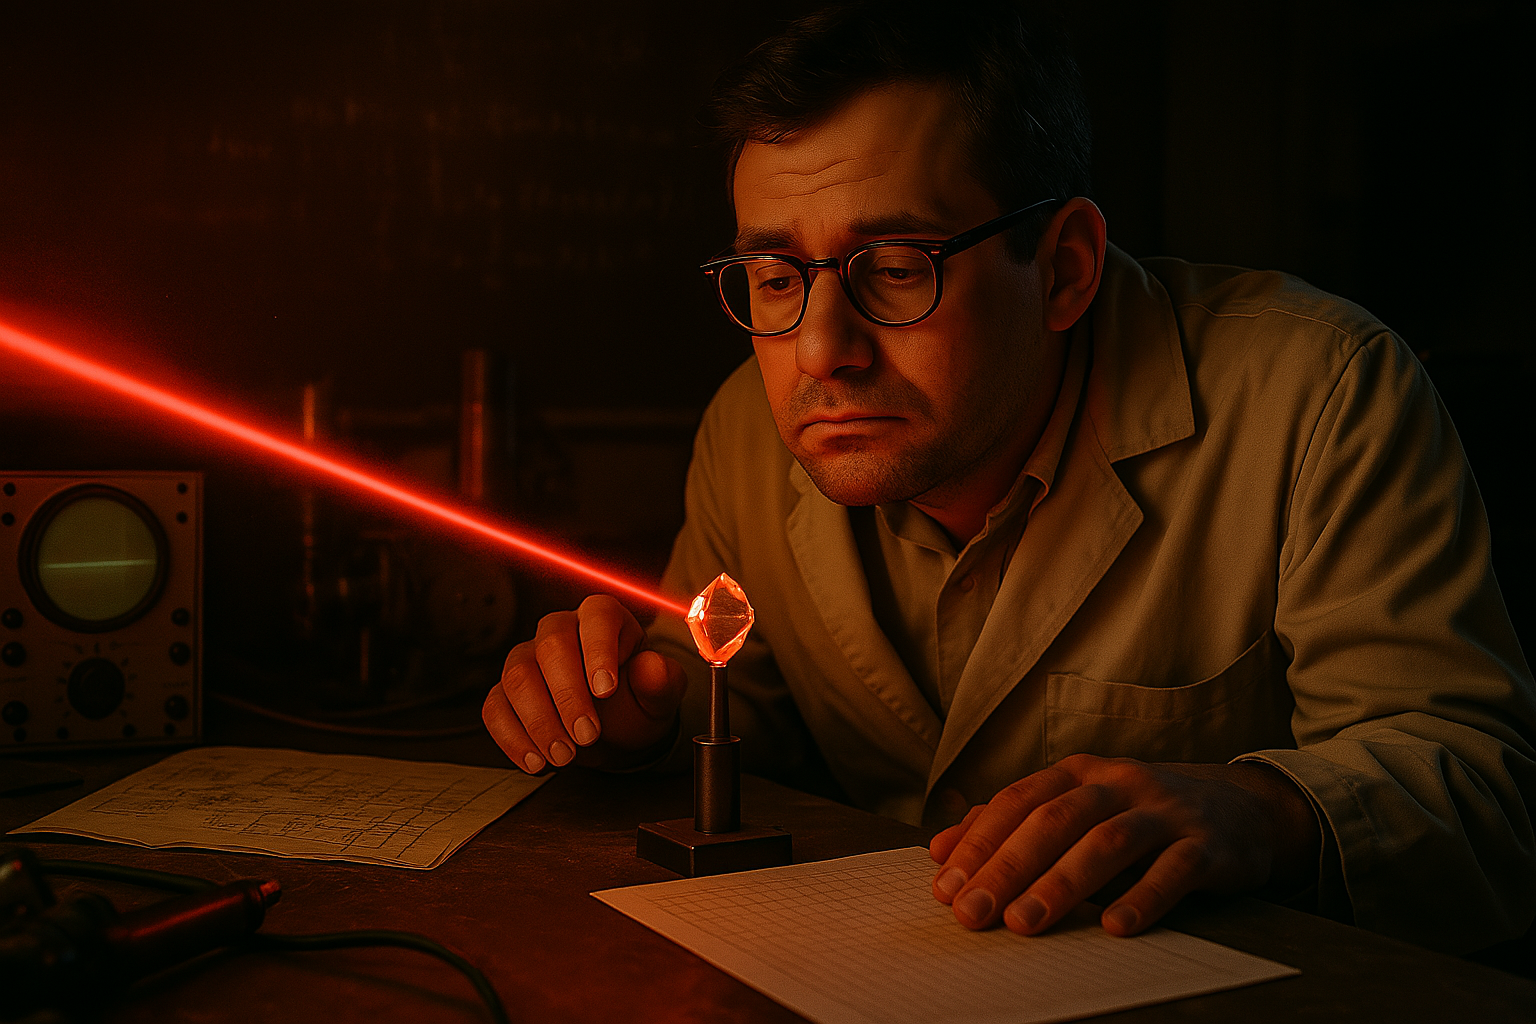
\includegraphics[width=0.9\textwidth]{Images/Copilot_20250706_224005.png}}
        \only<4>{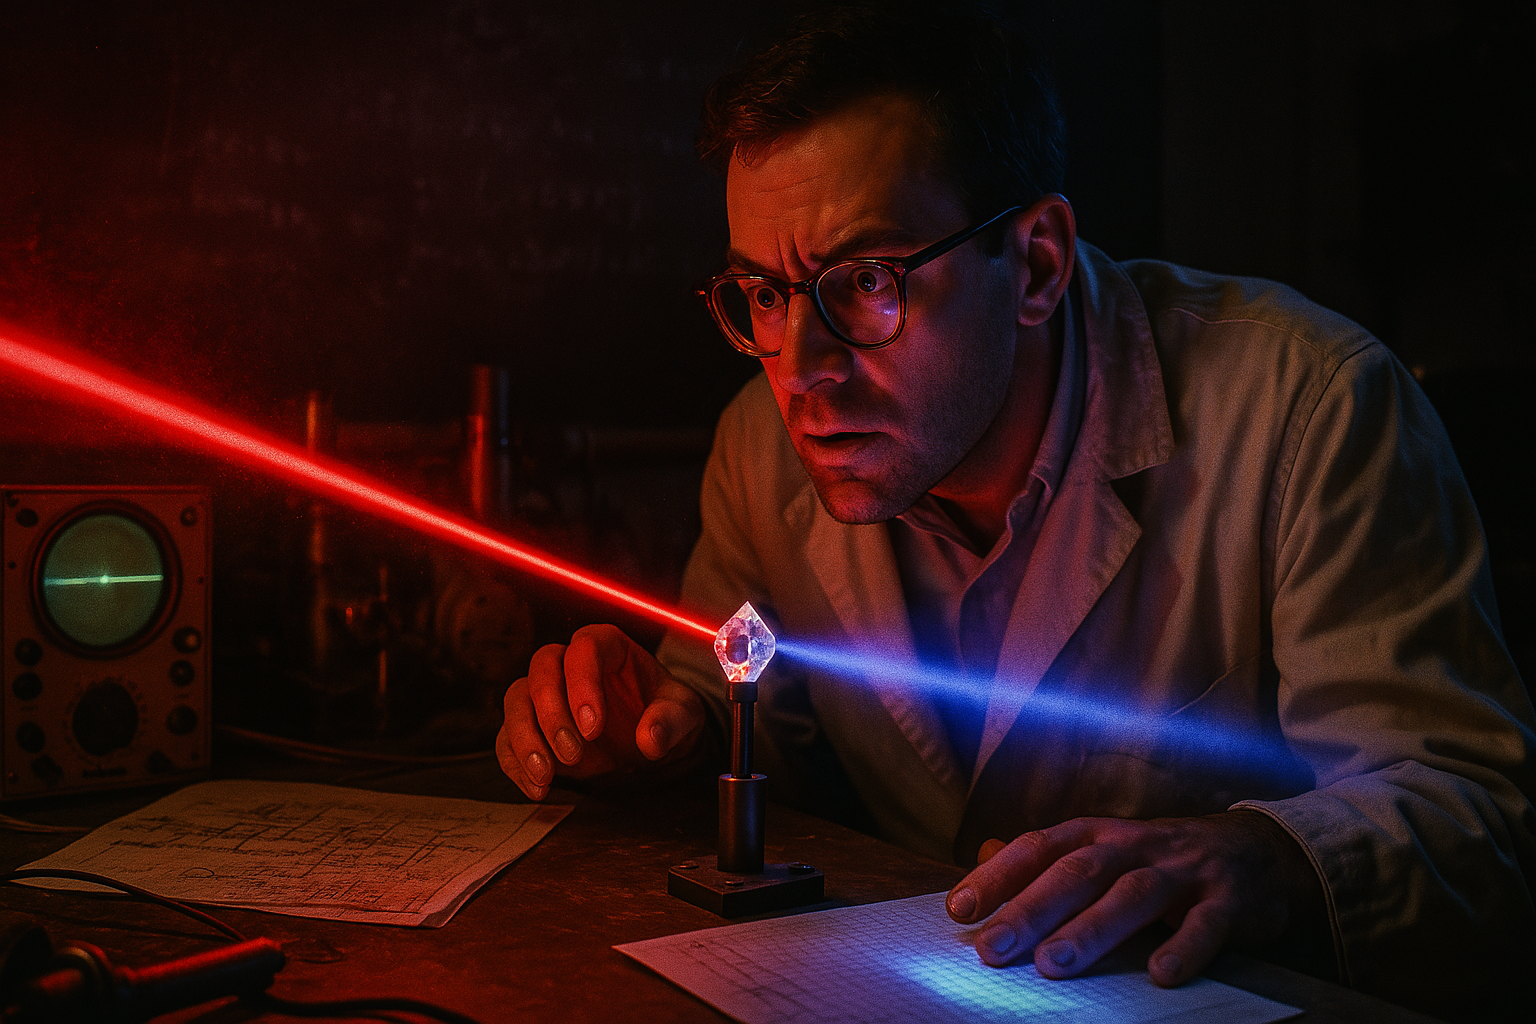
\includegraphics[width=0.9\textwidth]{Images/Copilot_20250706_215901.png}}
        \\ \tiny \textcolor{gray}{von: \citetitle{Copilot.2025} -- \citefield{Copilot.2025}{note}}
        \note{1961 beobachteten der Physiker Peter Franken und seine Mitarbeiter an der University of Michigan einen merkwürdigen Effekt: Bei der Bestrahlung eines Quarzkristalls mit einem der ersten Rubinlaser bestand das transmittierte Licht nicht nur aus Strahlung der Laserwellenlänge 694 nm, sondern es trat auch UV-Licht der halben Wellenlänge 347 nm aus. Das war die erste Beobachtung eines nichtlinearen Effektes, der Frequenzverdopplung,[2] und gilt als die Geburtsstunde der nichtlinearen Optik.}
    \end{frame}
   

    % % Appetizer Slide
    % \begin{frame}<handout:0>[noframenumbering, plain]{Appetizer}
    %     \centering
    %     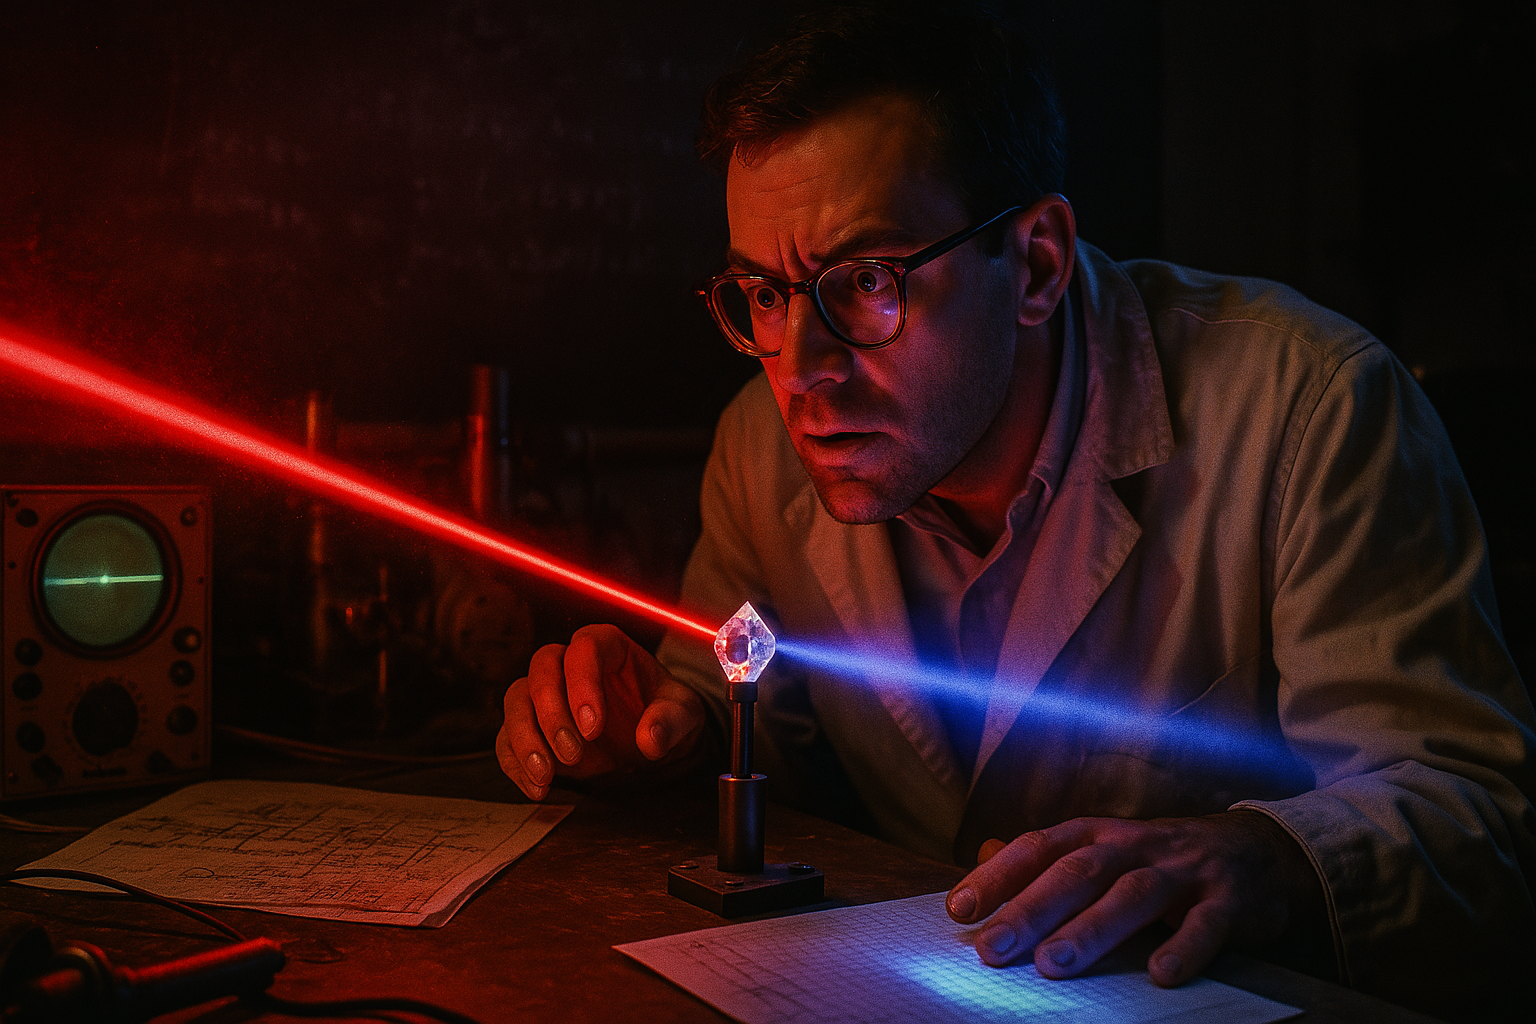
\includegraphics[width=\textwidth, height=0.9\textheight, keepaspectratio]{Images/Copilot_20250706_215901.png}
    %     \figciteweburl{Copilot.2025}
    %     % \vspace{0.5cm}
    %     % \begin{quote}
    %     %{Stellen Sie sich vor, ...}
    %     % \end{quote}
    % \end{frame}

    % Title Slide
    \begin{frame}[noframenumbering, plain]
        \vspace*{-0.6cm}
        \titlepage
        \vspace*{-1.6cm}
    \end{frame}
    
    % Table of Contents
    \begin{frame}<handout:0>{Gliederung} % Handout ausgeschaltet!!
      \setcounter{page}{1}      
        \tableofcontents
    \end{frame}
      \note{
        In dieser Präsentation beginnen wir mit den Grundlagen der nichtlinearen Optik. 
        Anschließend erkläre ich die Prinzipien der Frequenzverdopplung (SHG) und -verdreifachung (THG), 
        bevor wir auf das wichtige Konzept der Phasenanpassung eingehen. 
        Danach stelle ich einen typischen experimentellen Aufbau vor und zeige Beispiele sowie Anwendungen. 
        Am Ende folgt eine kurze Zusammenfassung. 
        Ziel ist es, dass Sie zunächst die grundlegenden Konzepte verstehen und dann nachvollziehen können, wie SHG und THG funktionieren.
      }
    
    % presentation slides
  
    \section{Einführung in die nichtlineare Optik}

\begin{frame}{Was ist nichtlineare Optik?}
  % Breite, niedrige Grafik oben
  \begin{center}
    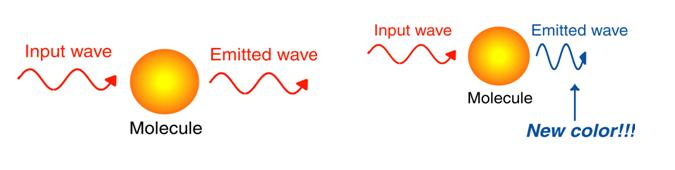
\includegraphics[width=0.6\textwidth]{Images/Fig.1 optics.jpeg}\\
    {\tiny Fig. 1: Linear (links) und nichtlineare (rechts) Wechselwirkung von Licht und Materie. Quelle: \cite{Science20NonlinearOptics2014}}
  \end{center}
  \vspace{0.2cm}
  \begin{columns}[T,onlytextwidth]
    \column{0.48\textwidth}
      \begin{itemize}
        \item \textbf{Lineare Optik:} $P \propto E$
        \item Materialantwort ist direkt proportional zum elektrischen Feld
        \item Gilt für alltägliche Lichtquellen (Sonne, Lampe)
      \end{itemize}
    \column{0.48\textwidth}
      \begin{itemize}
        \item \textbf{Nichtlineare Optik:} $P = \varepsilon_0(\chi^{(1)}E + \chi^{(2)}E^2 + \chi^{(3)}E^3 + \dots)$
        \item Zusätzliche Terme treten erst bei sehr hohen Intensitäten auf (starke Laser!)
      \end{itemize}
  \end{columns}
  \note{
    Die Grafik oben zeigt links die lineare, rechts die nichtlineare Antwort eines Mediums auf einfallendes Licht.\newline
    In der linearen Optik ist die Polarisation $P$ proportional zum Feld $E$. Erst bei sehr hohen Intensitäten (typisch: starke Laser) treten nichtlineare Terme auf.\newline
    Diese führen dazu, dass das Material neue Frequenzen erzeugt – z.B. die doppelte oder dreifache Frequenz des eingestrahlten Lichts.\newline
    Das ist die Grundlage für Second Harmonic Generation (SHG) und Third Harmonic Generation (THG).\newline
    Im Alltag bleibt die Optik fast immer linear, nichtlineare Effekte sind selten und erfordern spezielle Bedingungen.
  }
\end{frame}

\begin{frame}{Materialantwort: Wann tritt Nichtlinearität auf?}
  \begin{columns}[T,onlytextwidth]
    \column{0.38\textwidth}
      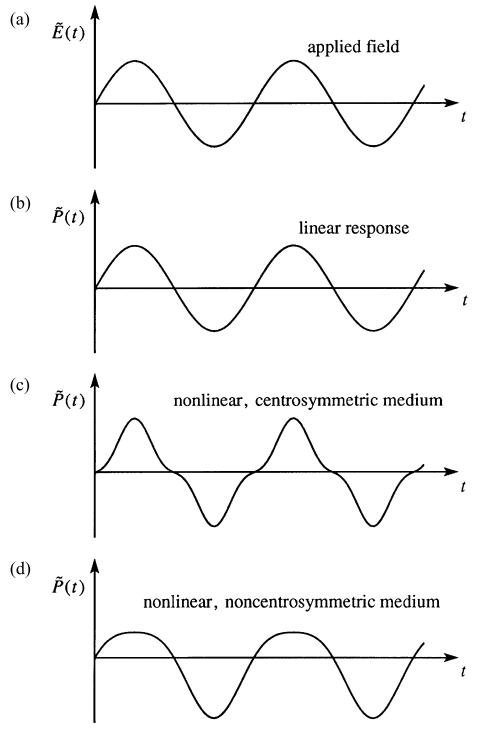
\includegraphics[height=0.8\textheight]{Images/Nonlinear response.png}
      \figciteweb{Boyd2020}
    \column{0.6\textwidth}
      \begin{itemize}
        \item Antwort eines Mediums auf sinusförmiges Feld
        \item Bei nichtlinearen Bedingungen: Verzerrte Schwingung $\rightarrow$ neue Frequenzen
        \item Zentrosymmetrie: gleich mehr
      \end{itemize}
  \end{columns}
  \note{
    Die Grafik zeigt, wie verschiedene Materialien auf ein sinusförmiges elektrisches Feld reagieren.\newline
    Nur Materialien ohne Inversionssymmetrie (z.B. viele Kristalle) zeigen eine starke nichtlineare Antwort ($\chi^{(2)} \neq 0$).\newline
    In zentrosymmetrischen Medien verschwindet $\chi^{(2)}$, sodass nur Effekte dritter Ordnung ($\chi^{(3)}$) wie THG möglich sind.\newline
    Die verzerrte Schwingung im rechten Teil der Grafik steht für die Entstehung neuer Frequenzen durch Nichtlinearität.
  }
\end{frame}
    
\section{Harmonische Generation}

% --- Folie 5: Zweitharmonische Generation (SHG) – Prinzip ---

\begin{frame}{Zweitharmonische Generation (SHG): Prinzip}
  \begin{columns}[T,onlytextwidth]
    \column{0.55\textwidth}
      \begin{itemize}
        \item Einfallende elektromagnetische Welle übt Kraft auf Elektronen (Dipolschwingung)
        \item Elektrisches Feld $E(t)$ versetzt Elektronen in periodische Bewegung
        \item Bewegung erzeugt zeitabhängige Polarisation $P(t)$
        \item Voraussetzung für SHG: Material nicht-zentrosymmetrisch ($\chi^{(2)} \neq 0$)
        \item $P^{(2)}(2\omega) = \varepsilon_0 \chi^{(2)} E(\omega)^2$
        \item $E(2\omega) \propto \chi^{(2)} [E(\omega)]^2$
        \item Energieerhaltung: $2\hbar\omega = \hbar(2\omega)$
      \end{itemize}
    \column{0.43\textwidth}
      %hier gif
      \begin{center}
      \animategraphics[autoplay,loop,width=0.95\columnwidth]{20}{Images/Electron_asymmetric_motion_animation/frame}{001}{060}
      \\[-1mm]{\tiny Elektronenbewegung im anharmonischen Potential: Neben der Grundfrequenz entstehen neue Frequenzen (Fourierpfeile: blau\:=\:linear, grün\:=\:SHG, rot\:=\:optische Rektoifikation). \figciteweburl{Sbyrnes3212014}}
      \end{center}
  \end{columns}
  \note{
    Bei der SHG verschmelzen zwei Photonen der Frequenz $\omega$ zu einem Photon mit $2\omega$.\newline
    Das funktioniert nur in Materialien ohne Inversionssymmetrie, weil nur dann $\chi^{(2)}$ ungleich null ist.\newline
    Formel: Die induzierte Polarisationskomponente bei 2ω ist $P^{(2)}(2\omega)=\varepsilon_0\chi^{(2)}E(\omega)E(\omega)$, daraus folgt für das elektrische Feld $E(2\omega)\propto \chi^{(2)}[E(\omega)]^2$. (Folie: Grafik oder Formel zeigen.)\newline
    Die Elektronenbewegung im anharmonischen Potential ist nicht mehr sinusförmig – dadurch entstehen neue Frequenzen (siehe Fourierpfeile in der Animation).\newline
    Die Formel $P^{(2)}(2\omega) = \varepsilon_0 \chi^{(2)} E(\omega)^2$ beschreibt die Polarisationskomponente bei $2\omega$.\newline
    Energieerhaltung: Zwei Photonen werden zu einem mit doppelter Energie.
  }
\end{frame}

% --- Folie 6: Zweitharmonische Generation (SHG) – Beispiele & Bedingungen ---

\begin{frame}{Zweitharmonische Generation (SHG): Beispiele \& Bedingungen}
  \begin{columns}[T,onlytextwidth]
    \column{0.55\textwidth}
      \begin{itemize}
        \item Typische Kristalle: BBO, KTP, KDP, LBO
        \item Benötigt starke, gepulste Laser (z.B. Nd:YAG 1064 nm $\rightarrow$ 532 nm grün)
        \item Effizienz oft gering, exakte Ausrichtung nötig
        \item SHG historisch erstmals 1961 mit Rubinlaser beobachtet (Franken)
        \item \textbf{Praxis:} Quadratische Abhängigkeit der SHG-Intensität von der Eingangsleistung
      \end{itemize}
    \column{0.43\textwidth}
      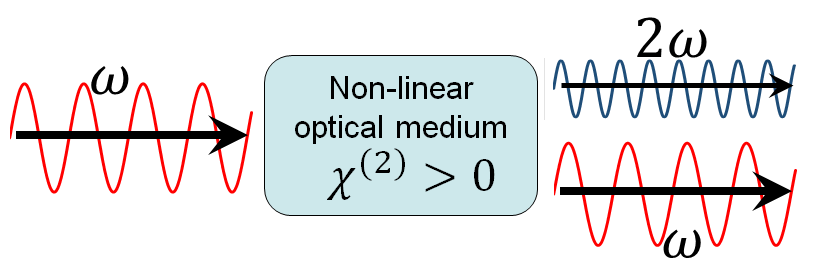
\includegraphics[width=0.95\textwidth]{Images/Schematic_of_the_SHG_conversion_of_an_excited_wave_in_a_non-linear_medium.png}\\
      {\tiny Schematische Darstellung: Einfallende Welle erzeugt zweite Harmonische im nichtlinearen Medium. \figciteweburl{BPAegirsson2017}}
  \end{columns}
  \note{
    Für effiziente SHG braucht man starke, meist gepulste Laser und spezielle Kristalle ohne Inversionssymmetrie.\newline
    Typische Materialien sind BBO, KTP, KDP oder LBO.\newline
    Die Effizienz ist oft gering, daher ist eine exakte Ausrichtung und Phasenanpassung wichtig.\newline
    Praktisch wird z.B. aus einem 1064 nm Nd:YAG-Laser durch SHG ein 532 nm grüner Strahl erzeugt.\newline
    Die schematische Grafik zeigt, wie im Kristall aus der Grundwelle die zweite Harmonische entsteht.
  }
\end{frame}


\begin{frame}{Energieerhaltung und Photonenprozesse}
  \begin{columns}[T,onlytextwidth]
    \column{0.38\textwidth}
      % SHG & THG Formeln
      \vspace{1.6cm}
      \begin{itemize}
        \item \textbf{SHG:} $2\,\hbar\omega \rightarrow \hbar(2\omega)$
        \item \textbf{THG:} $3\,\hbar\omega \rightarrow \hbar(3\omega)$
        \item \textbf{Energieerhaltung:} $n\,\hbar\omega = \hbar(n\omega)$
      \end{itemize}
    \column{0.6\textwidth}
      \centering
      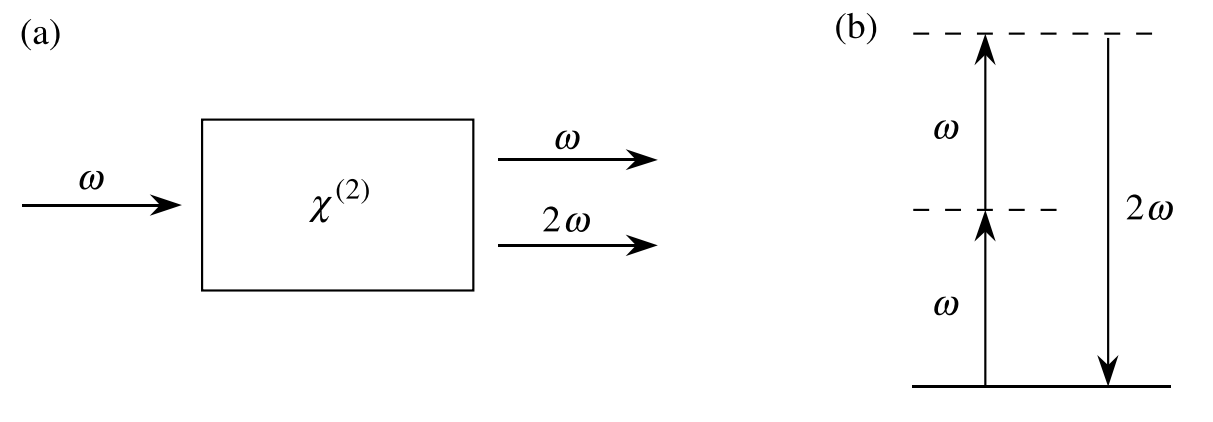
\includegraphics[width=0.98\textwidth]{Images/shg.png}\\
      \small SHG: $\omega \rightarrow 2\omega$\\
      {\tiny aus: \citeauthortitle{Boyd2020}}
  \end{columns}

  \vspace{0.2cm}

  \begin{itemize}
    
    \item Multiphotonenprozesse erfordern hohe Intensitäten
    \item Wahrscheinlichkeit nimmt mit der Ordnung ab
    \item Gerade Ordnungen (z.B. SHG) nur in nicht-zentrosymmetrischen Materialien
  \end{itemize}

  \note{
    Die Folie zeigt die grundlegenden Photonenprozesse bei der harmonischen Generation. Links sehen wir die Second Harmonic Generation (SHG): Zwei Photonen der Frequenz $\omega$ verschmelzen zu einem Photon mit $2\omega$. Rechts ist die Third Harmonic Generation (THG) dargestellt: Drei Photonen mit $\omega$ werden zu einem Photon mit $3\omega$.\newline
    Entscheidend ist die Energieerhaltung: Die Summe der einfallenden Photonenenergien entspricht der Energie des erzeugten Photons.\newline
    Solche Prozesse treten nur bei sehr hohen Lichtintensitäten auf, wie sie typischerweise mit Lasern erreicht werden.\newline
    Die Wahrscheinlichkeit für diese Prozesse nimmt mit der Ordnung ab – also ist SHG viel wahrscheinlicher als THG.\newline
    Wichtig: Gerade Ordnungen wie SHG sind nur in nicht-zentrosymmetrischen Materialien möglich, während ungerade Ordnungen wie THG auch in zentrosymmetrischen Medien auftreten können.
  }
\end{frame}

\begin{frame}{Drittharmonische Generation (THG)}
  \begin{columns}[T,onlytextwidth]
    \column{0.52\textwidth}
      \begin{itemize}
        \item \textbf{THG:} Drei Photonen $\omega$ erzeugen ein Photon $3\omega$ (Frequenzverdreifachung)
        \item \textbf{Formel:} $P^{(3)}(3\omega) = \varepsilon_0 \chi^{(3)} E(\omega)^3$
        \item $E(3\omega) \propto \chi^{(3)} [E(\omega)]^3$
        \item \textbf{Voraussetzung:} Kein Symmetriebruch nötig ($\chi^{(3)}$ in allen Materialien)
        \item THG ist meist schwächer als SHG
        \item Effektiver an Grenzflächen oder bei Brechungsindexgradienten (z.B. THG-Mikroskopie)
      \end{itemize}
    \column{0.46\textwidth}
      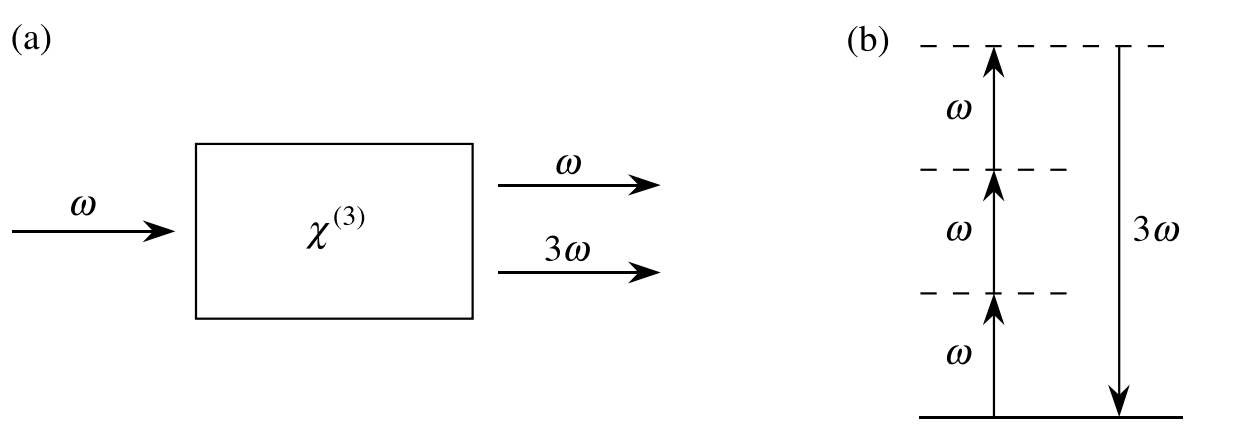
\includegraphics[width=0.95\textwidth]{Images/thg.png}\\
      {\tiny Schematische Darstellung: Drei Photonen $\omega$ erzeugen ein Photon $3\omega$. \figciteweb{Boyd2020}}
  \end{columns}
  \vspace{0.2cm}
  \begin{itemize}
    \item \textbf{Energieerhaltung:} $3\hbar\omega = \hbar(3\omega)$
    \item \textbf{Praxis:} THG tritt auch in Flüssigkeiten und Gasen auf, nicht nur in Kristallen
  \end{itemize}
  \note{
    Bei der Drittharmonischen Generation (THG) verschmelzen drei Photonen der Frequenz $\omega$ zu einem Photon mit $3\omega$.\newline
    Im Gegensatz zur SHG ist kein Symmetriebruch nötig: $\chi^{(3)}$ ist in allen Materialien vorhanden, daher kann THG auch in zentrosymmetrischen Medien (z.B. Flüssigkeiten) auftreten.\newline
    Die Formel $P^{(3)}(3\omega) = \varepsilon_0 \chi^{(3)} E(\omega)^3$ beschreibt die Polarisationskomponente bei $3\omega$.\newline
    THG ist meist schwächer als SHG, da der Effekt dritter Ordnung ist.\newline
    Besonders effektiv ist THG an Grenzflächen oder in Bereichen mit Brechungsindexgradienten, z.B. in der THG-Mikroskopie.\newline
    Die schematische Grafik zeigt, wie drei Photonen zu einem Photon mit dreifacher Frequenz verschmelzen.
  }
\end{frame}

\begin{frame}{Nichtlineare Suszeptibilität}
  \begin{columns}[T,onlytextwidth]
    \column{0.48\textwidth}
      \centering
      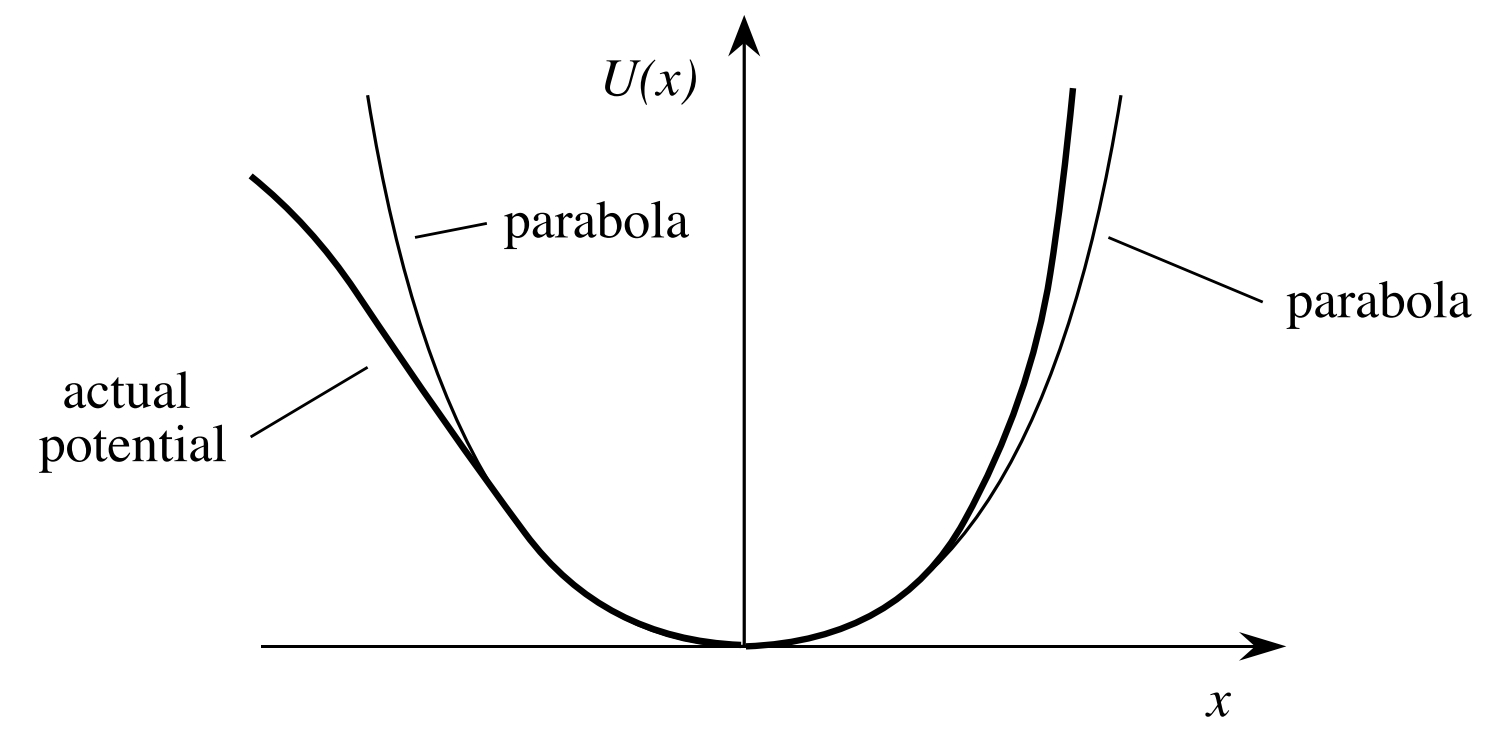
\includegraphics[width=0.7\textwidth]{Images/pot_noncentrosym.png}\\
      {\tiny Nicht-zentrosymmetrisch (\cite{Boyd2020})}
      \begin{itemize}
        \item \textbf{\(\chi^{(2)}\):} Second-order (SHG), nur in nicht-zentrosymmetrischen Materialien
        \item \textbf{\(\chi^{(3)}\):} Third-order (THG), in allen Materialien möglich
        \item \textbf{Größenordnungen:} \(\chi^{(2)}\) typ. $10^{-12}$ bis $10^{-8}$ m/V, \(\chi^{(3)}\) noch kleiner
      \end{itemize}
    \column{0.48\textwidth}
      \centering
      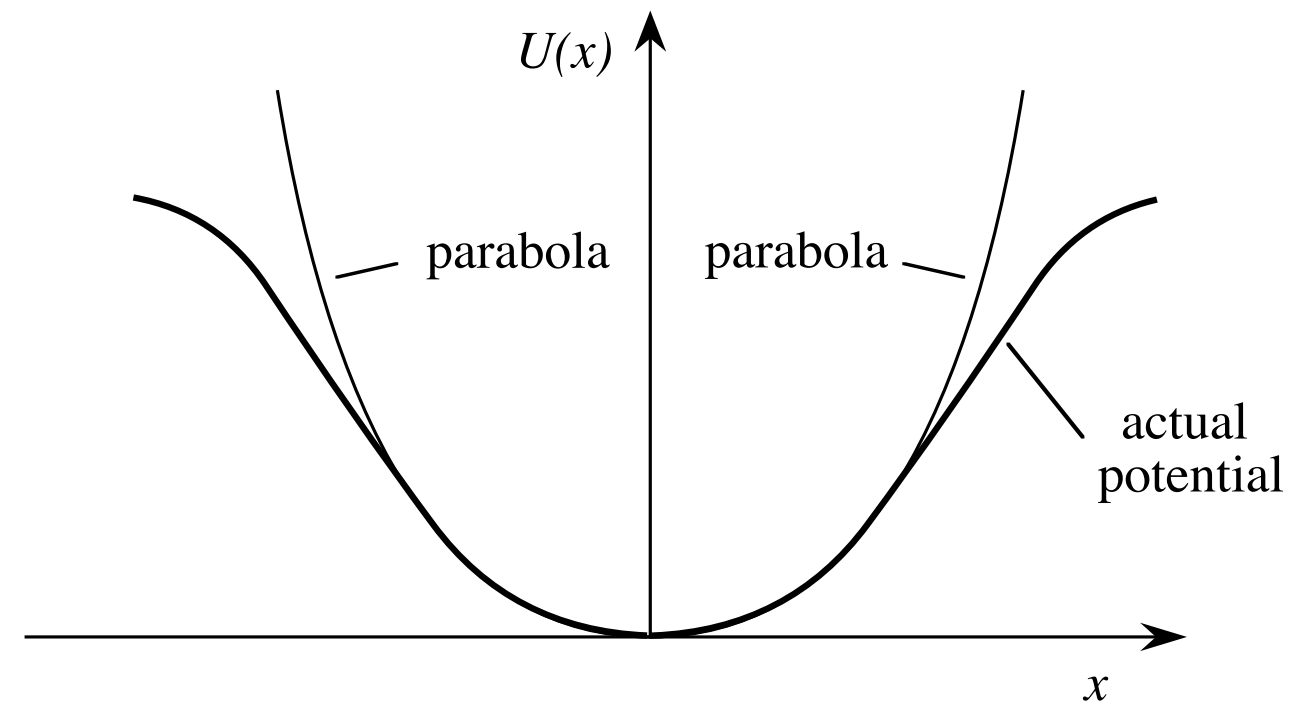
\includegraphics[width=0.7\textwidth]{Images/pot_centrosym.png}\\
      {\tiny Zentrosymmetrisch (\cite{Boyd2020})}
      \begin{itemize}
        \item Symmetrie entscheidet, welche Terme auftreten:
        \begin{itemize}
          \item Kein Inversionszentrum: \(\chi^{(2)} \neq 0\), z.B. viele Kristalle
          \item Mit Inversionszentrum: \(\chi^{(2)} = 0\), nur \(\chi^{(3)}\) bleibt
        \end{itemize}
      \end{itemize}
  \end{columns}

  \note{
    Die Folie erklärt, warum nicht alle Materialien für SHG geeignet sind.\newline
    Oben sieht man zwei Potentialtöpfe: links ohne Inversionssymmetrie – hier können gerade und ungerade Terme auftreten, also sowohl \(\chi^{(2)}\) als auch \(\chi^{(3)}\). rechts mit Inversionssymmetrie – hier verschwindet \(\chi^{(2)}\), nur \(\chi^{(3)}\) bleibt.\newline
    Das ist der Grund, warum SHG nur in nicht-zentrosymmetrischen Kristallen beobachtet wird, während THG in allen Materialien möglich ist.\newline
    Die Werte für \(\chi^{(2)}\) sind meist sehr klein, aber in bestimmten Kristallen ausreichend groß für effiziente Frequenzkonversion.\newline
    Symmetrie ist der Schlüssel: Sie entscheidet, welche nichtlinearen Terme auftreten können!
  }
\end{frame}




    % Thank You Slide
    \begin{frame}{Vielen Dank der Aufmerksamkeit!}
      \begin{center}
          \Huge Fragen?
      \end{center}
  \end{frame}

% Black slide
\begin{frame}<handout:0>[plain, noframenumbering]
  \begin{tikzpicture}[remember picture, overlay]
      \fill[black] (current page.south west) rectangle (current page.north east);
  \end{tikzpicture}
\end{frame}

  \begin{frame}<handout:0>[noframenumbering, plain, allowframebreaks]{Anhang}
      \begin{minipage}{0.4\textwidth}
        \textbf{Title}
        \begin{itemize}
          \item point one
          \item point two
          \item point three
        \end{itemize}
      \end{minipage}
      \hfill
      \begin{minipage}{0.58\textwidth}
        asfd
      \end{minipage}
      
    \pagebreak
      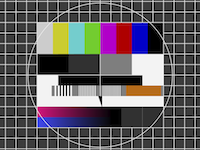
\includegraphics[height=0.9\textheight, width=\linewidth, keepaspectratio]{Images/test_pattern.png}%\caption{C Amsler, T DeGrand et al 2017 - Quark Model.jpg}
      \figcite{C.Amsler.2017}
    
    \end{frame}


    
    % Bibliography    
  \begin{frame}[allowframebreaks, noframenumbering, plain]{Literaturverzeichnis}
   \printbibliography%[nottype=unpublished]
    \end{frame}

\end{document}
